%This is a Latex file.
\documentclass[12pt]{article}
\usepackage{latexsym,fancyhdr,amsmath,amsfonts,amsthm,dsfont}
\usepackage{amssymb}
\usepackage{tikz}
\usetikzlibrary{graphs}
\usepackage{graphicx} 

% margins are relative to the default of 1 in
%\topmargin       -0.2 in

\topmargin        -0.2 in
\textheight       8.4 in
\oddsidemargin    0 in     % this is for pages 1, 3, 5, ...
\evensidemargin   0 in     % and this for 2, 4, 6, ...
\textwidth        6.5 in
%\headheight       15 in     % we won't have a running head, nor
\headsep          .35 in     % any extra space between head and text

%\parindent 0pt

\pagestyle{fancy} \lhead{\sf MTH 317} \chead{\sf Homework 3}
\rhead{\sf Rayana Gottschall} \lfoot{} \cfoot{} \rfoot{}

\newcommand{\C}{\mathds{C}}
\newcommand{\I}{\mathds{I}}
\newcommand{\N}{\mathds{N}}
\newcommand{\Q}{\mathds{Q}}
\newcommand{\R}{\mathds{R}}
\newcommand{\Z}{\mathds{Z}}
\begin{document}
\begin{enumerate}
\item[2.20]  Show that if G is a connected graph that is not regular, then G contains adjacent vertices
 u and v such that deg(u) $\neq$ deg(v).
\begin{proof}
Since $G$ is not regular, there exist vertices $x$ and $y$ with $\deg(x) \neq \deg(y)$.
Because $G$ is connected, there is a path $P : x=v_0,v_1,\dots,v_k=y$ between them. 

\textbf{Case 1: ($x$ and $y$ are adjacent)} If $k=1$, then $x$ and $y$ are adjacent and we are done. 


\textbf{Case 2: ($x$ and $y$ are not adjacent)} If $k \geq 2$, consider the sequence of degrees
\[
\deg(v_0), \deg(v_1), \dots, \deg(v_k).
\]
This sequence begins with $\deg(v_0)=\deg(x)$ and ends with $\deg(v_k)=\deg(y)$, which are different. 
Therefore, there must exist some index $i$ with $0 \leq i < k$ such that $\deg(v_i) \neq \deg(v_{i+1})$. 
Since $v_i$ and $v_{i+1}$ are adjacent in $G$, this gives the desired pair of adjacent vertices of unequal degree.

Thus, in all cases $G$ contains adjacent vertices $u,v$ with $\deg(u)\neq\deg(v)$.
\end{proof}

\noindent\textbf{2.22}
\begin{center}
    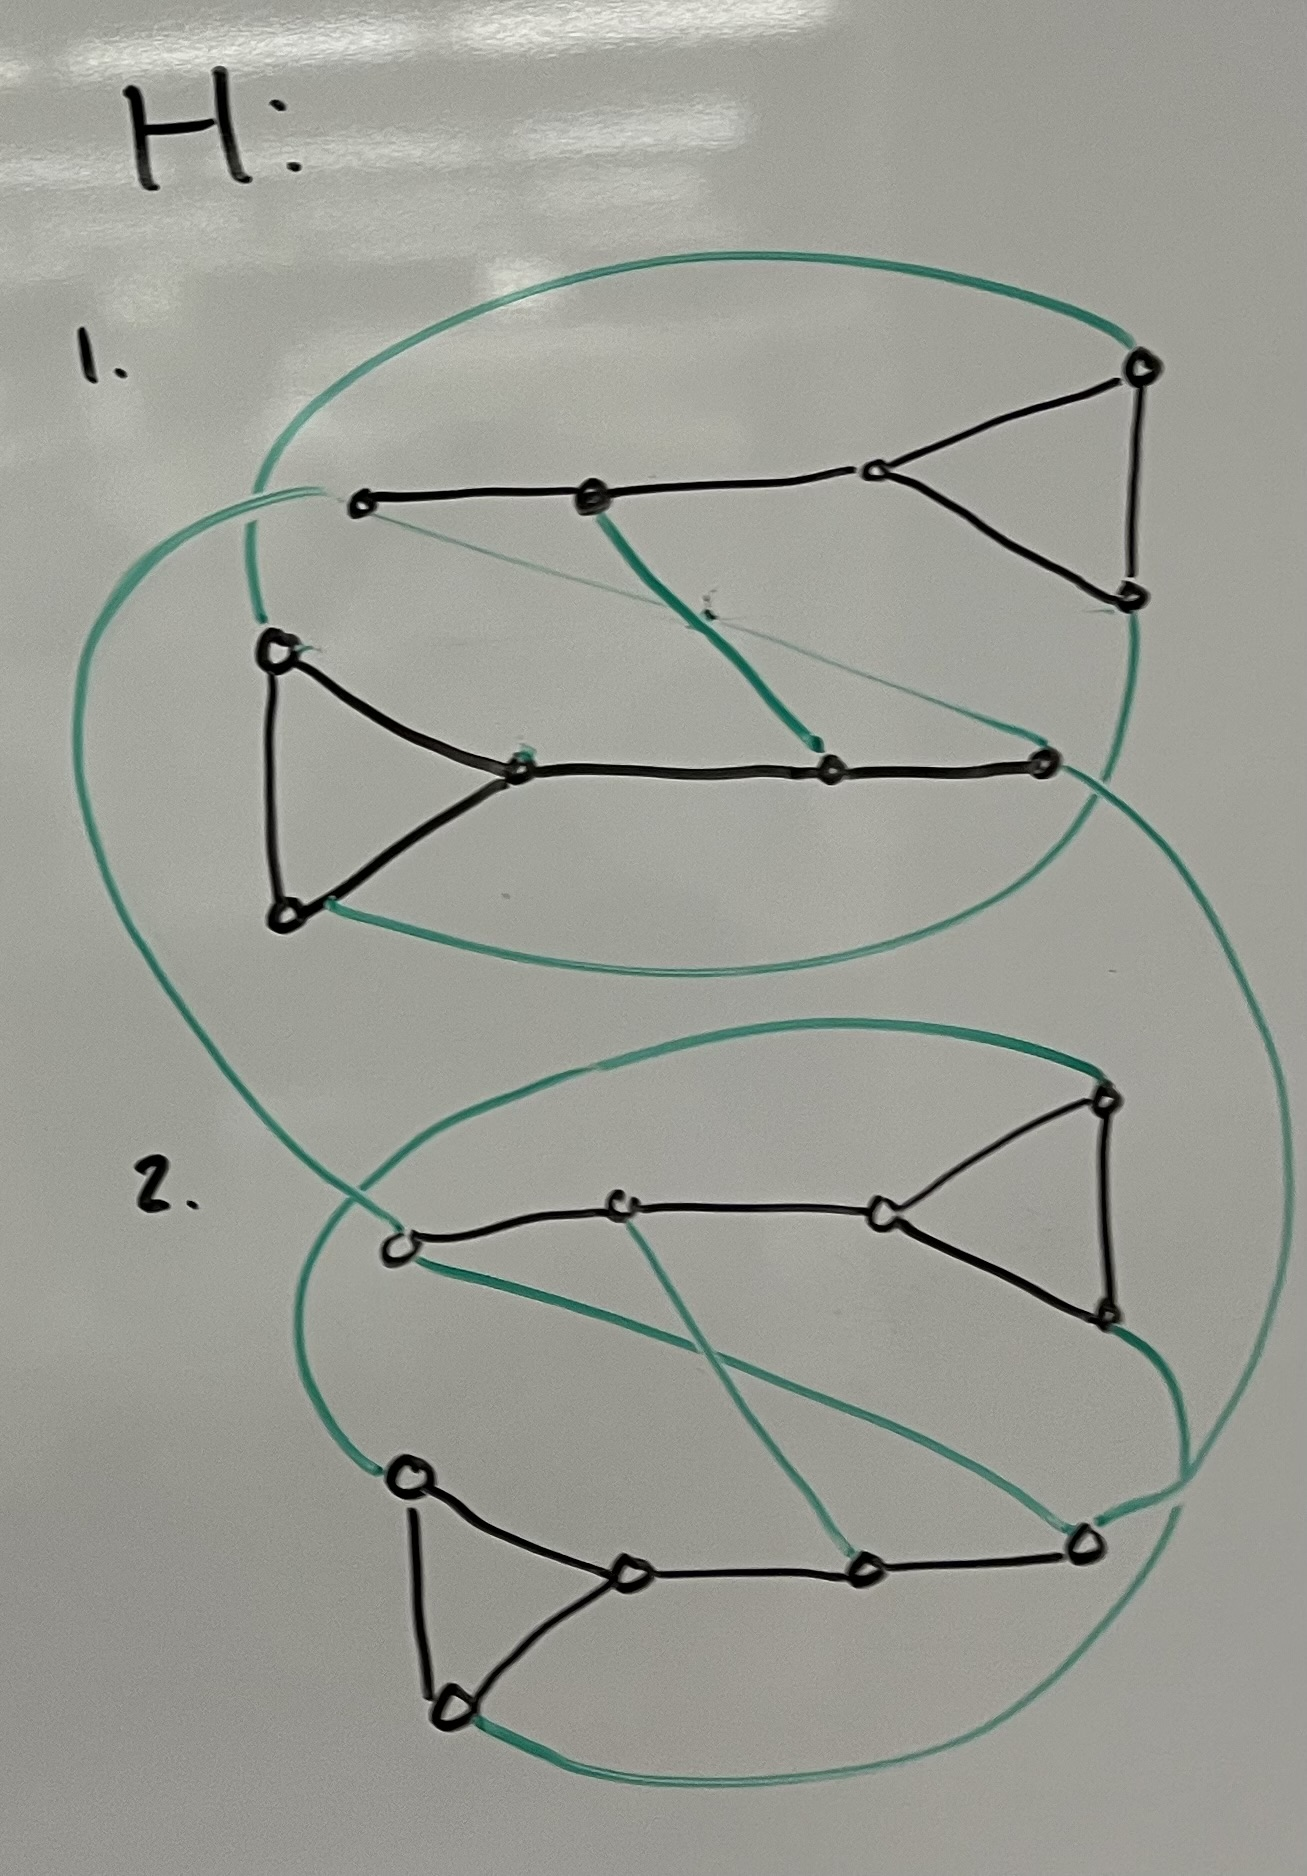
\includegraphics[width=0.5\textwidth]{IMG_1782.jpg}
    \newline
    Theorem 2.7: $r$ $\geq$ $\delta$(G). Here, r = 3 and $\delta$(G) = 3, so the theorem holds.
    Order = 20
\end{center}

\item[2.26] 
\item[a] Show that a graph G is regular if and only if its complement is regular.
\begin{proof}
    ($\Rightarrow$) Suppose G is r-regular. Then every vertex has degree r. 
    The degree of a vertex v in $\overline{G}$ is given by deg(v) = n - 1 - deg(v) in G, where n is the order of G.
    Since every vertex in G has degree r, every vertex in $\overline{G}$ has degree n - 1 - r. Therefore, $\overline{G}$ is (n - 1 - r)-regular.
    \newline
    ($\Leftarrow$) Suppose $\overline{G}$ is s-regular. Then every vertex has degree s. 
    The degree of a vertex v in G is given by deg(v) = n - 1 - deg(v) in $\overline{G}$, where n is the order of G.
    Since every vertex in $\overline{G}$ has degree s, every vertex in G has degree n - 1 - s. Therefore, G is (n - 1 - s)-regular.
    \newline
    Thus, a graph G is regular if and only if its complement is regular.
\end{proof} 


\item[b] Show that if G and $\overline{G}$ are r-regular for some nonnegative integer r, then G has odd order.
\begin{proof}
    Let the order of G be n. Then the degree of each vertex in $\overline{G}$ is n - 1 - r. Since $\overline{G}$ is r-regular, we have n - 1 - r = r. 
    Therefore, n - 1 = 2r, and n = 2r + 1. Since r is a nonnegative integer, 2r is even, and adding 1 gives an odd number. 
    So, n is odd, and G has odd order.
\end{proof}

\item[2.32] Determine if the following sequences are graphic. If so, construct a graph.
\item[b] 
    $S_1$: 6,3,3,3,3,2,2,2,2,1,1
    \newline
    $S_2$: 2,2,2,2,2,2,1,1,1,1
    \newline
    $S_3$: 2,2,2,1,1,1,1,1,1
    \newline
    $S_4$: 1,1,1,1,1,1,1,1. Here, we have an even number of 1s, and can recognize this is graphic.
    \newline
    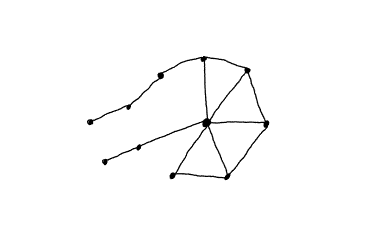
\includegraphics{grapha.png}


\item[d] 
    $S_1$: 7,5,4,4,4,3,2,1
    \newline
    $S_2$: 4,3,3,3,2,1,0
    \newline
    $S_3$: 2,2,2,1,1
    \newline
    $S_4$: 1,1,1,1. Here, we have an even number of 1s, and can recognize this is graphic.
    \newline
    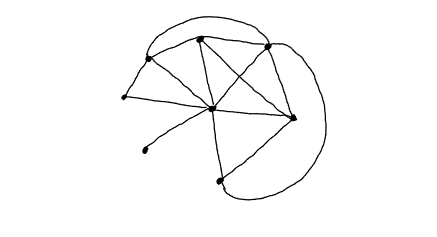
\includegraphics{graphd.png}



\item[2.33] Prove that for every integer x with 0 $\leq$ x $\leq$ 5, the sequence x,1,2,3,5,5 is not graphical.
\begin{proof}
    The sum of all degrees must be even. Here, the sum is x + 16. So x must be even. Therfore, x $\neq$ 1, 3, 5.
    That leaves 0, 2, and 4. We can use Theorem 2.10 to show each case is not graphical.
    \newline
    x = 0:
    $S_1$: 1,2,3,5,5 or 5,5,3,2,1. This is not graphical because there is a vertex of degree 5, but only 4 other vertices.
    \newline
    x = 2:
    $S_1$: 2,1,2,3,5,5 or 5,5,3,2,2,1
    \newline
    $S_2$: 4,3,1,1,0. This is not graphical because there is a vertex of degree 4, but only 3 other vertices.
    \newline
    x = 4: 
    \newline
    $S_1$: 4,1,2,3,5,5 or 5,5,4,3,2,1    
    \newline
    $S_2$: 4,3,2,1,0. This is not graphical because there is a vertex of degree 4, but only 3 other vertices.
    \newline
    Therefore, for every integer x with 0 $\leq$ x $\leq$ 5, the sequence x,1,2,3,5,5 is not graphical. 
\end{proof} 


\end{enumerate}
\end{document}
